%% example.tex
%% Copyright 2012 Bruno Menegola
%
% This work may be distributed and/or modified under the
% conditions of the LaTeX Project Public License, either version 1.3
% of this license or (at your option) any later version.
% The latest version of this license is in
%   http://www.latex-project.org/lppl.txt
% and version 1.3 or later is part of all distributions of LaTeX
% version 2005/12/01 or later.
%
% This work has the LPPL maintenance status ‘maintained’.
%
% The Current Maintainer of this work is Bruno Menegola.
%
% This work consists of all files listed in MANIFEST
%
%
% Description
% ===========
%
% This is an example latex document to build presentation slides based on
% the beamer class using the Inf theme.

\documentclass{beamer}

\usepackage[T1]{fontenc}
\usepackage[brazil]{babel}
\usepackage[utf8]{inputenc}
\usepackage{graphicx}
\usepackage{booktabs}
\usepackage{palatino}
\usepackage{hyphenat}
\usepackage{listings}
\usepackage{caption}
\renewcommand{\raggedright}{\leftskip=0pt \rightskip=0pt plus 0cm}

% Choose the Inf theme
\usetheme{Inf}

% Define the title with \title[short title]{long title}
% Short title is optional
\title[]
      {Otimizando StarVZ para carga de grandes volumes de dados}

% Optional subtitle
\subtitle{Especialização em Big Data \& Data Science}

\date{13 de Setembro de 2019}

% Author information
\author{Alexandre Miyazaki  \\ Orientador: Lucas Mello Schnorr}
\institute{Instituto de Informática --- UFRGS\\}

\begin{document}

% Command to create title page
\InfTitlePage

\begin{frame}
  \frametitle{Agenda}
  \tableofcontents
\end{frame}

\section{Introdução}
\begin{frame}
\frametitle{StarVZ}
  \begin{itemize}
   \item StarVZ é um arcabouço de análise de desempenho cujo objetivo é auxiliar 
na verificação de hipóteses sobre aplicações baseadas em tarefas.
   \item Este domínio carece de ferramentas de visualização voltadas para este 
tipo de aplicação, devido a dominância do modelo predecessor (BSP - 
\textit{Bulk-Synchronous Parallel}).
  \item Ele é separado em duas fases sendo uma de pré-processamento e outra de 
visualização.
  \end{itemize}
\end{frame}

\begin{frame}
 \frametitle{StarVZ - Fases}
 \begin{figure}[H]
  \centerline{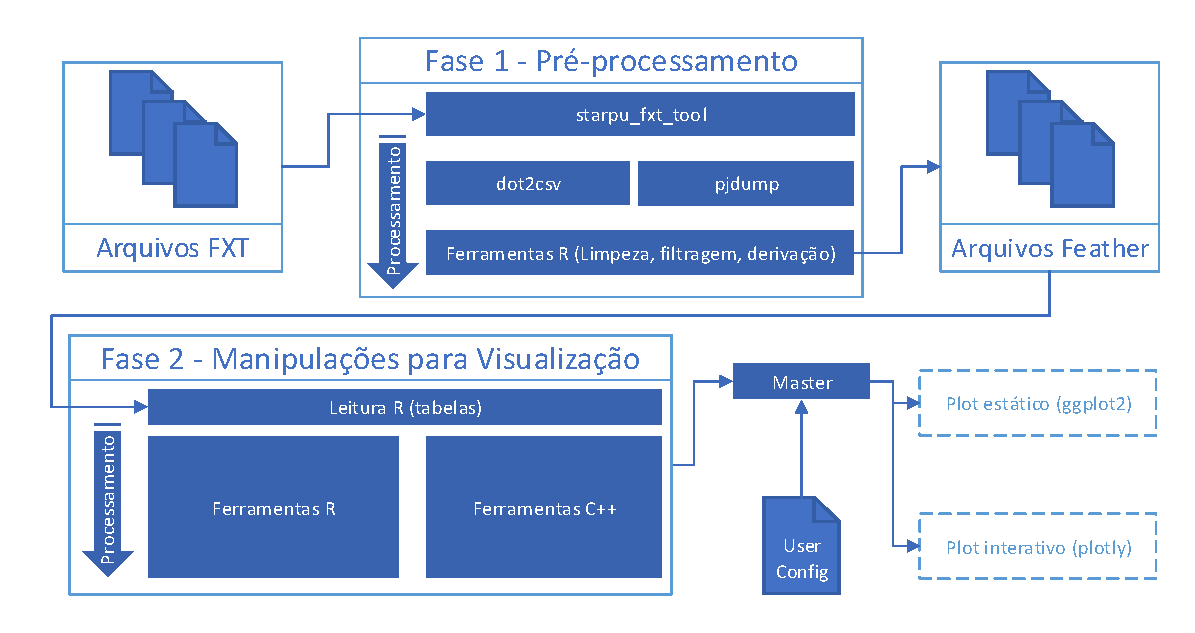
\includegraphics[width=1\textwidth]{./img/all-proc.pdf}}
  \label{fig:hadoop}
  \end{figure}
\end{frame}

\begin{frame}
\frametitle{Motivação/Trabalhos Relacionados}
  \begin{itemize}
   \item Em estudos anteriores, analisou-se logs com 18 GB, derivados de uma 
pequena execução envolvendo poucos nós computacionais.
   \item A primeira fase do StarVZ levou cerca de 32 minutos para processar.
   \item Tal desempenho pode inviabilizar o uso do StarVZ para cargas de 
grandes volumes de dados.
   \item Houve uma tentativa de otimizar o fluxo do StarVZ com 
\texttt{Drake}, biblioteca cujo foco é executar apenas as fases necessárias de 
um fluxo de processamento e análise.
  \item Não foi possível otimizar o fluxo com \texttt{Drake}, devido a cache de 
resultados intermediários da biblioteca ter um uso intensivo de disco.
  \end{itemize}
\end{frame}

\begin{frame}
 \frametitle{Objetivo}
\textbf{Viabilizar o uso do StarVZ para análise de grandes volumes de dados 
utilizando ferramentas voltadas para este fim.}
\end{frame}


\section{Ferramentas}

\begin{frame}
 \frametitle{Hadoop}
 \begin{figure}[H]
  \centerline{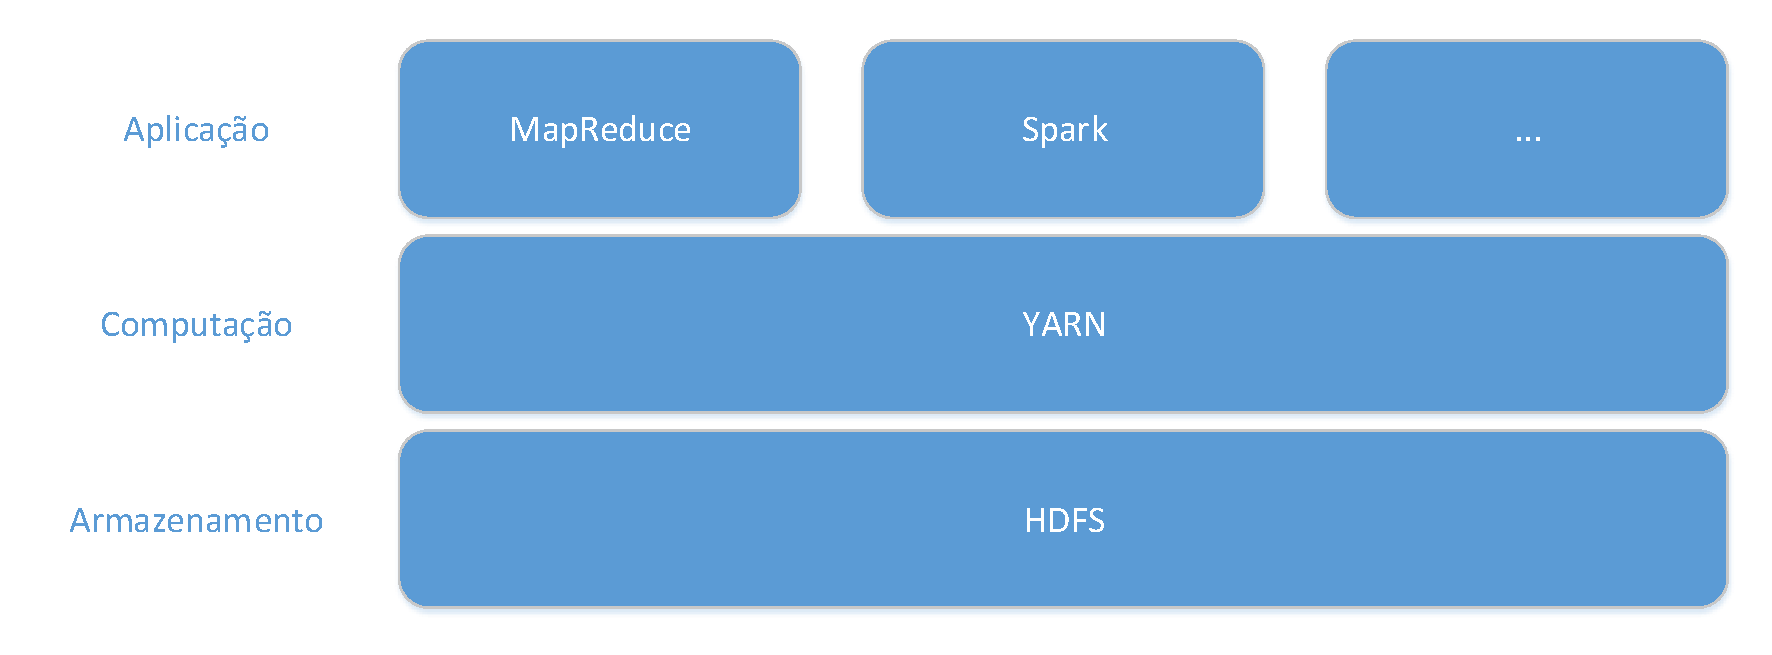
\includegraphics[width=1\textwidth]{./img/hadoop-layers.pdf}}
 \end{figure}
  \begin{itemize}
  \item Arcabouço que permite o processamento de grandes volumes de dados.
  \item Organização em camadas.
  \end{itemize}
\end{frame}

\begin{frame}
 \frametitle{Spark}
 \begin{figure}[ht]
  \centerline{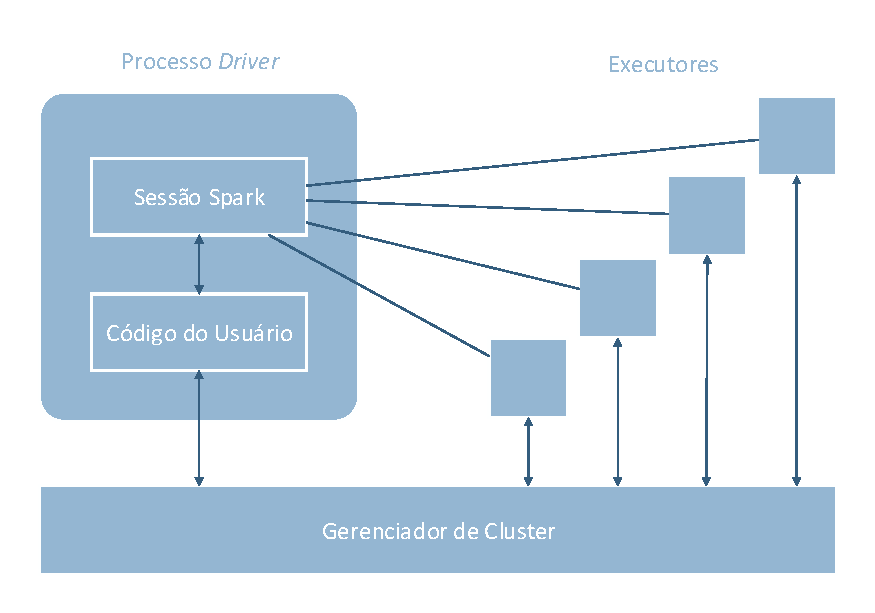
\includegraphics[width=0.7\textwidth]{./img/spark-arch.pdf}}
  \end{figure}
  \begin{itemize}
  \item \textit{Engine} unificada + conjunto de bibliotecas para processamento 
de dados distribuídos.
  \item Utilizado via biblioteca \texttt{sparklyr}.
  \end{itemize}
\end{frame}


\section{Implementação}
\begin{frame}
 \frametitle{Abordagem}
 \begin{itemize}
  \item Otimizar processamento de tabelas, não o fluxo da aplicação.
  \item Focado nas ferramentas R, que consistem em \textasciitilde 40\% do 
tempo total da primeira fase.
  \item Utilizar equivalências entre \texttt{sparklyr} e \texttt{dplyr}.
  \item Processo foi facilitado pois a \texttt{sparklyr} é baseada na {dplyr}.
 \end{itemize}
\end{frame}

\begin{frame}
 \frametitle{Fluxo da Aplicação}
 \begin{figure}[H]
 \centerline{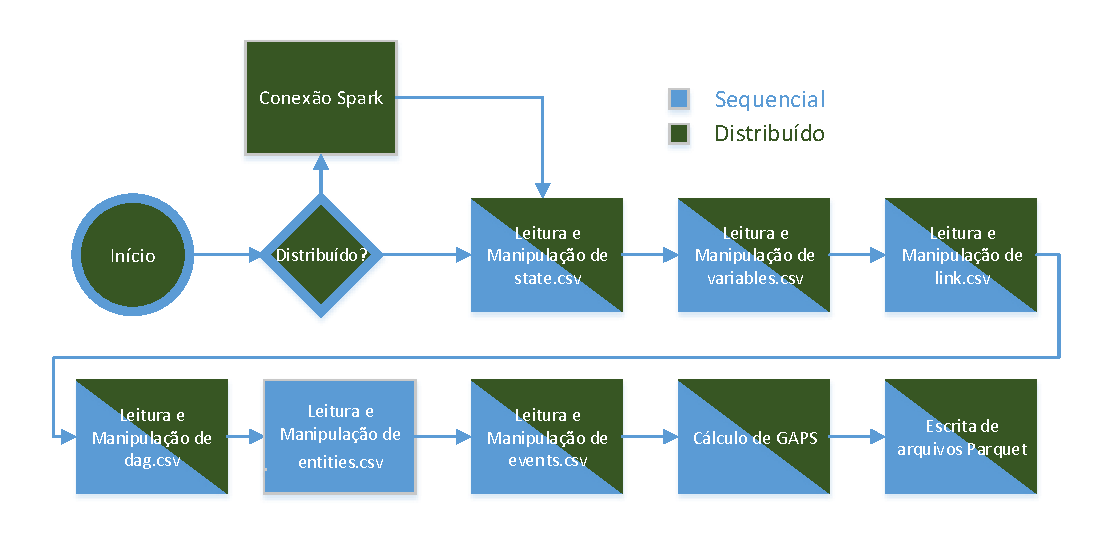
\includegraphics[width=1\textwidth]{./img/applicationflow.pdf}}
 \end{figure}
\end{frame}

\begin{frame}
 \frametitle{Equivalências}
 \begin{table}[H]
  \centering
  \small
  \begin{tabular}{c c} \toprule
  \textbf{Operação \texttt{dplyr}}  &  \textbf{Operação \texttt{sparklyr}}\\ 
  \midrule
  distinct	& unique  \\
  sort		& sdf\_sort \\
  gsub		& regexp\_replace\\
  rbind		& union\_all\\
  grepl		& rlike\\
  separate	& ft\_regex\_tokenizer + sdf\_separate\_column       \\
  \bottomrule
  \end{tabular}
  \end{table}
\end{frame}

\begin{frame}
 \frametitle{Validação}
 \begin{itemize}
  \item Conjunto de dados pequeno (835 MB).
  \item Objetivo foi validar se o resultado da versão modificada era 
equivalente ao da original.
  \item Realizada por tabela.
  \item Diversos agrupamentos realizados em suas colunas.
  \item Comparação de resultados entre ambas as execuções.
 \end{itemize}
\end{frame}


\section{Avaliação e Resultados}
\begin{frame}
 \frametitle{Projeto Experimental}
  \begin{figure}[ht]
  \hspace*{-0.5cm}
  \centerline{
  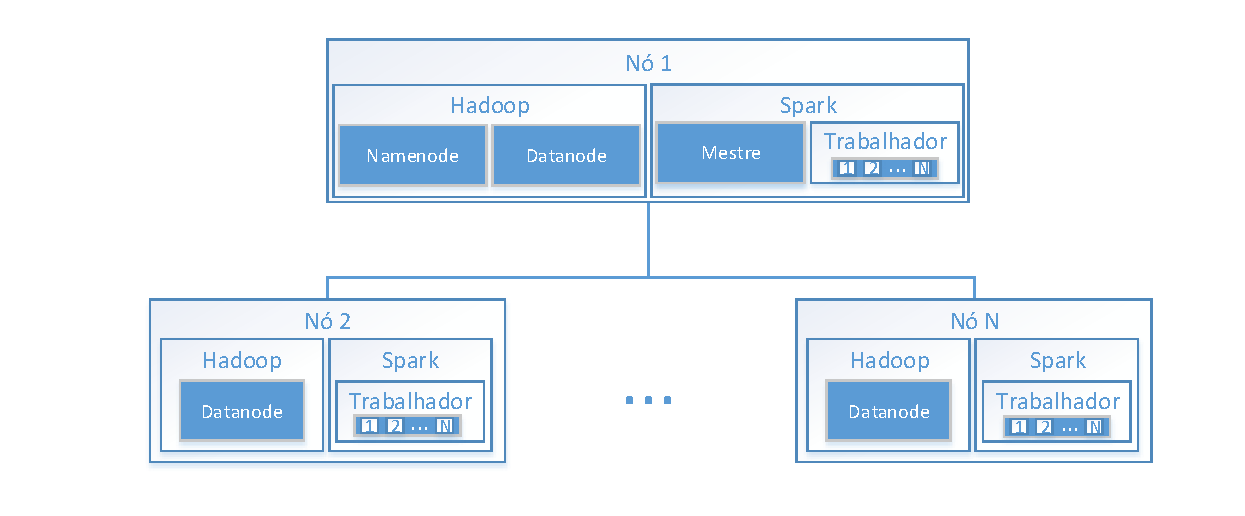
\includegraphics[scale=0.65]{./img/experiments_arch.pdf}}
  \legend{Organização de ferramentas nos nós.}
  \end{figure}
\end{frame}

\begin{frame}
 \frametitle{Ambiente e Metodologia}
 \begin{columns}[T] % align columns
  \begin{column}{.55\textwidth}
 \begin{table}[H]
  \centering
  \small
  %\footnotesize
  \begin{tabular}{l c} \toprule
  \textbf{Parâmetro}  &  \textbf{Configuração} \\ 
  \midrule
  Processador     & 2 x Intel Xeon, 2,5 GHz\\
  Núcleos Físicos    & 16  \\
  Núcleos Lógicos   & 32   \\
  Memória       & 64 GB DDR3  \\
  Rede	      &  10 Gigabit \\
  \bottomrule
  \end{tabular}
  \end{table}
  \end{column}%
  \hfill%
  \begin{column}{.41\textwidth}
  \begin{itemize}
   \item Testes com 1 nó com versão sequencial.
   \item Testes com 1, 2 e 3 nós, instanciando 15 executores por nó na versão 
distribuída.
   \item \textasciitilde30 repetições por teste.
   \item Entrada de 12 GB.
  \end{itemize}
  \end{column}%
  \end{columns}
\end{frame}


\begin{frame}
 \frametitle{Resultados}
 \begin{itemize}
  \item Speedups de respectivamente 2,10x, 3,23x e 3,86x em relação a aplicação 
original.
 \end{itemize}
 \begin{figure}[ht]
  \centerline{
  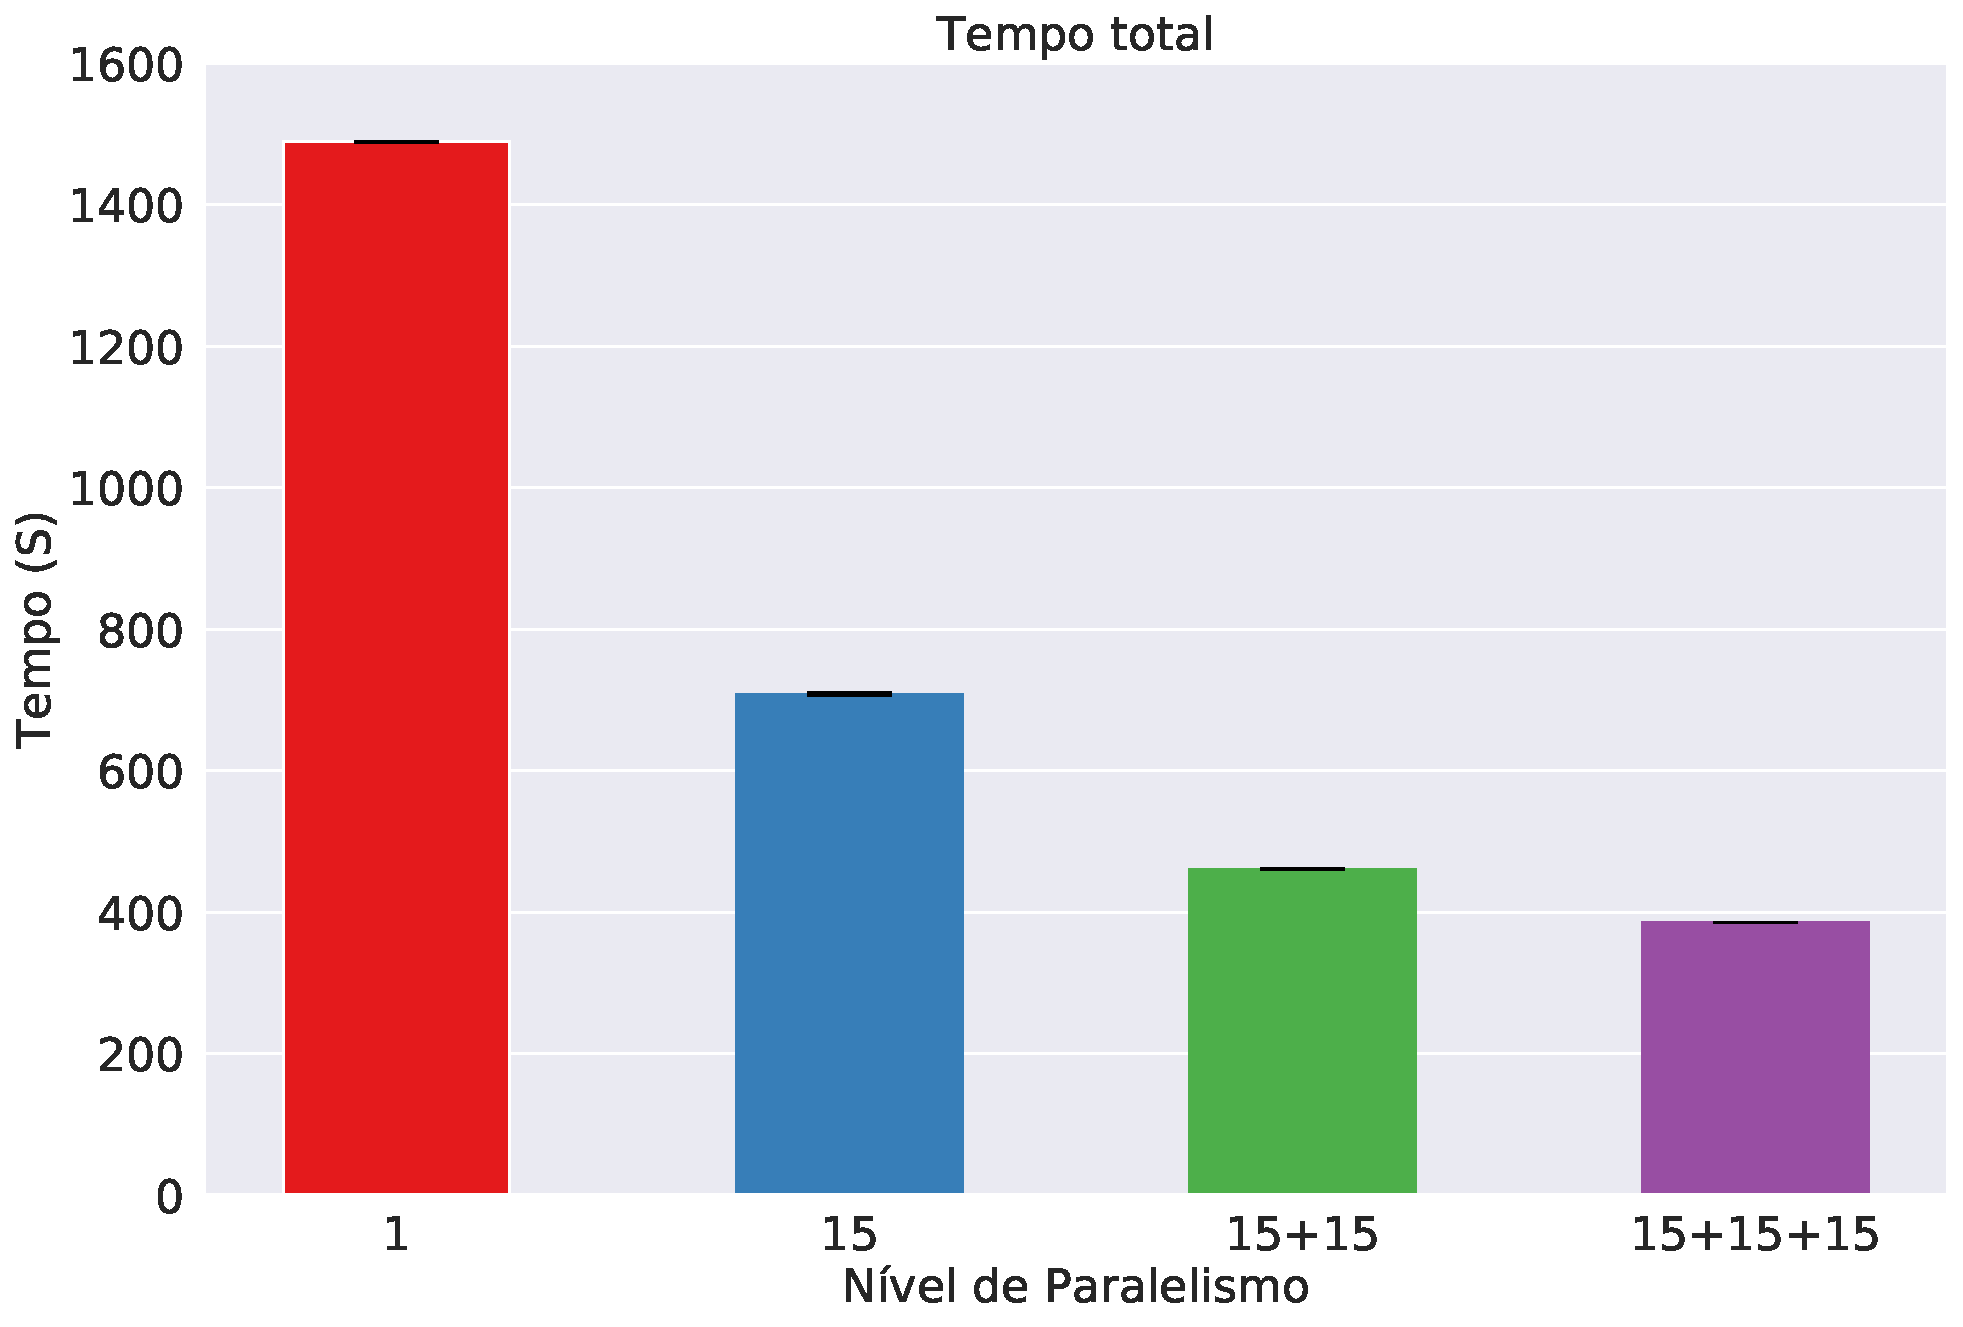
\includegraphics[width=0.8\textwidth]{./img/total.pdf}}
  \legend{Teste de escalabilidade.}
  \end{figure}
\end{frame}


\begin{frame}
 \frametitle{Resultados}
  \begin{table}[ht]
  \begin{tabular}{l c c c c} \toprule
  \textbf{Etapa}  & \textbf{1} & \textbf{15} & \textbf{15+15} & 
  \textbf{15+15+15}\\ 
  \midrule
  State		& 873.31 & 215.93 & 142.15 & 119.20\\
  Variable  	& 210.77 & 21.17  & 10.44  & 7.50 \\
  Link      	& 8.93   & 4.59   & 3.84   & 3.53 \\
  DAG        	& 69.14  & 10.10  & 7.58   & 6.76 \\
  Entities	& 3.07   & 2.42   & 2.31   & 2.30 \\
  Events		& 89.87  & 42.68  & 22.65  & 15.91\\
  GAPS		& 71.51  & 154.03 & 110.83 & 95.22\\
  Write		& 162.19 & 211.06 & 125.40 & 102.87\\
  \end{tabular}
  \end{table}
  \begin{itemize}
   \item Quatro grupos identificados nos resultados por etapas.
  \end{itemize}
\end{frame}

\begin{frame}
 \frametitle{Resultados}
  \begin{figure}[ht]
  \centerline{
  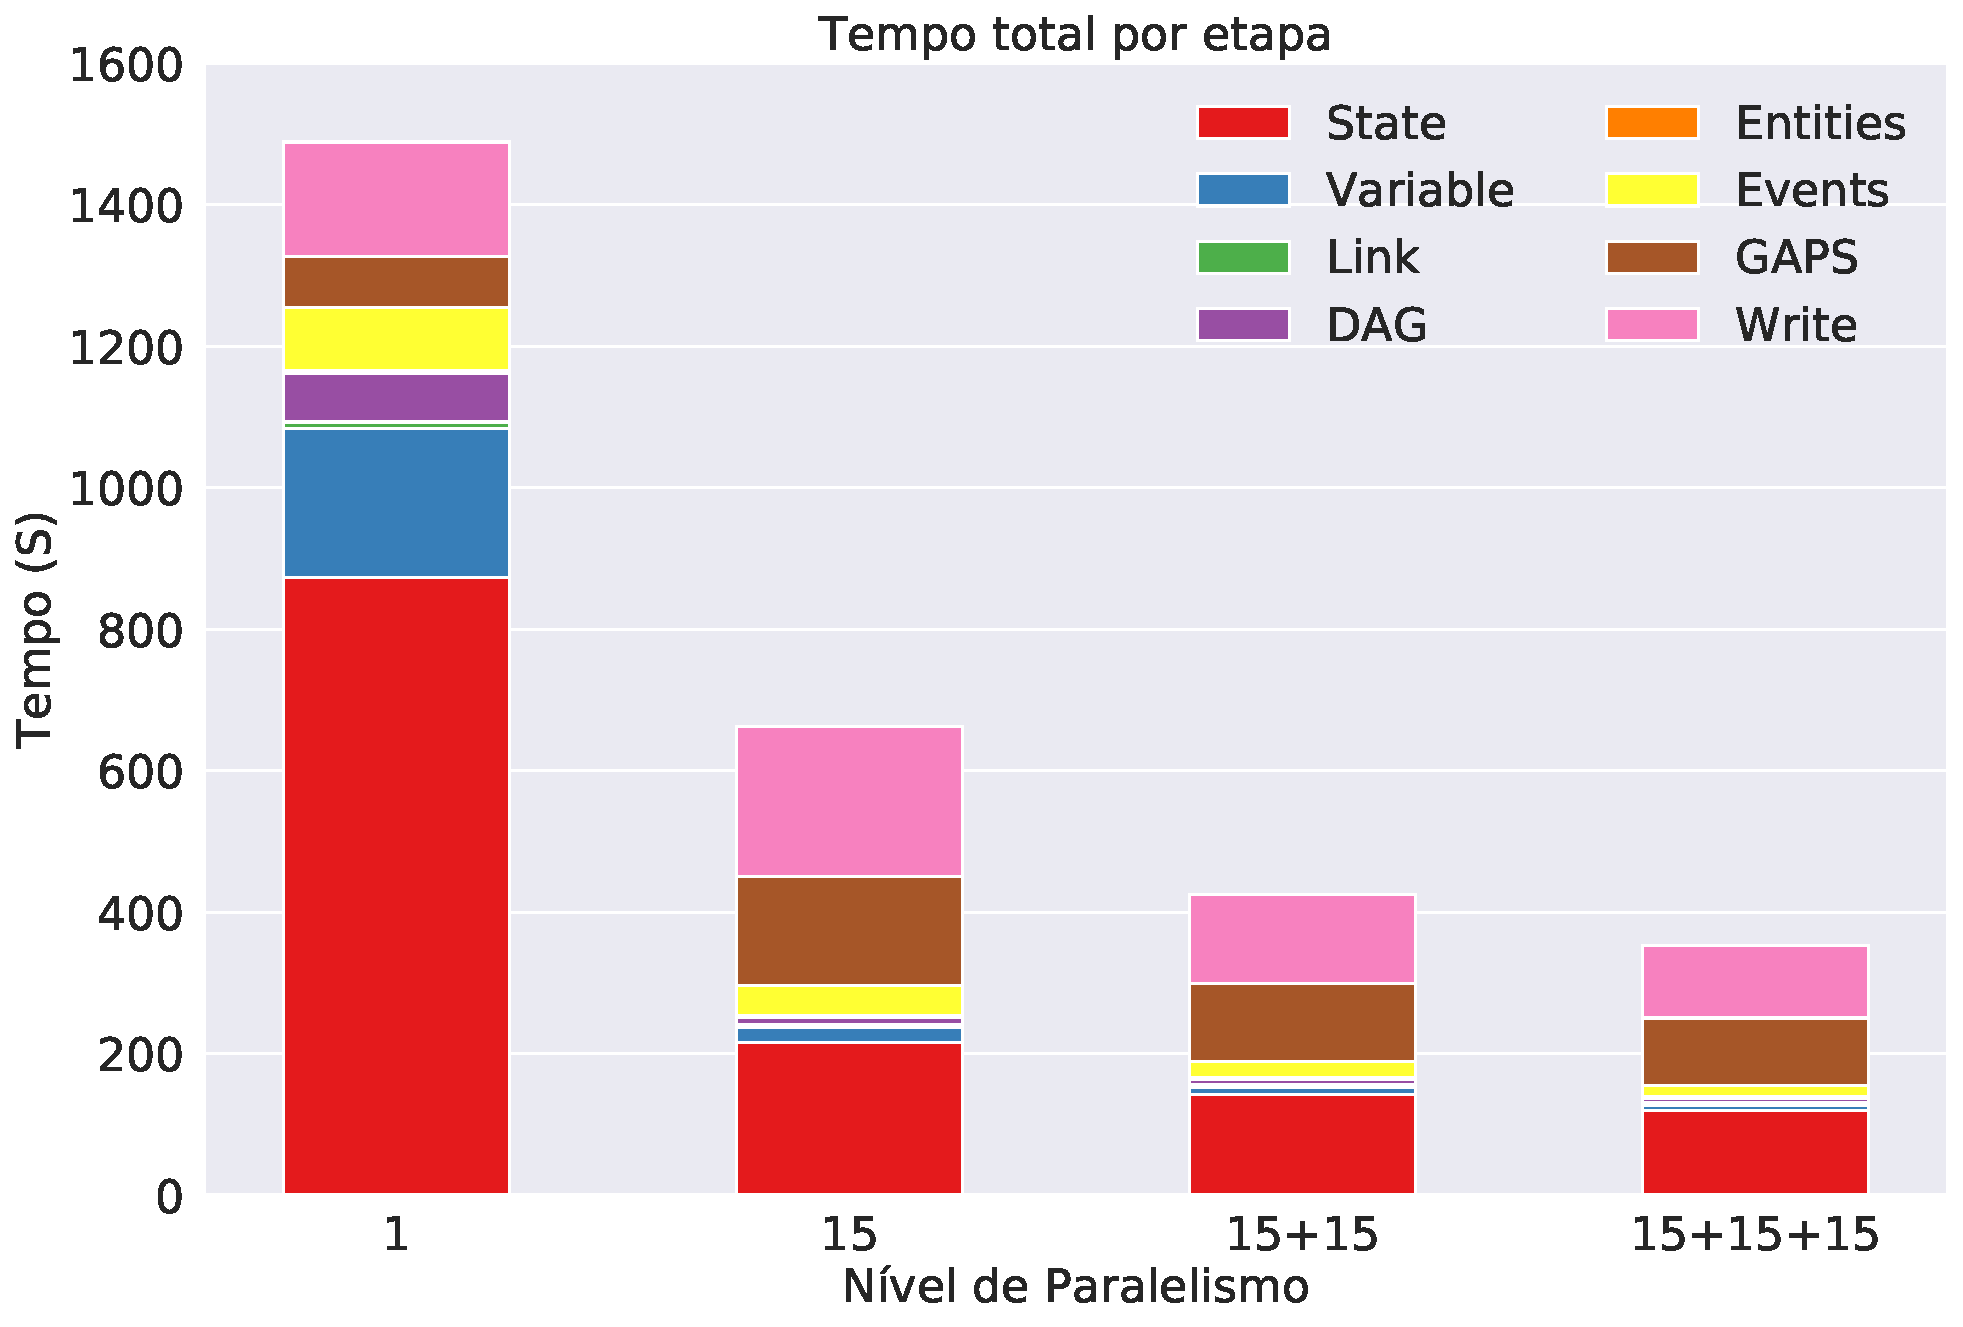
\includegraphics[width=0.8\textwidth]{./img/total_step.pdf}}
  \legend{Teste de escalabilidade.}
  \end{figure}
  \begin{itemize}
   \item Quatro grupos identificados nos resultados por etapas.
  \end{itemize}
\end{frame}



\section{Conclusão}

\begin{frame}
 \frametitle{Realizações}
 \begin{itemize}
  \item Apenas com as equivalências entre \texttt{dplyr} e \texttt{sparklyr}, 
foi possível atingir \emph{speedups} totais de:	
    \begin{itemize}
      \item 2,10x com 1 nó / 15 executores;
      \item 3,23x com 2 nós / 30 executores;
      \item 3,86x com 3 nós / 45 executores.
    \end{itemize}
  \item Portanto, conseguimos otimizar a etapa mais custosa do arcabouço StarVZ.
  \item Vale salientar que com o formato de execução distribuído, o StarVZ é 
capaz de processar mais dados do que o tamanho de memória de uma única máquina.
 \end{itemize}
\end{frame}

\begin{frame}
 \frametitle{Trabalhos Futuros}
 \begin{itemize}
  \item Testes com com volume ainda maior de dados.
  \item Testes com arquivos de registro de outras aplicações.
  \item Incorporação ao pacote StarVZ.
  \item Otimização de demais etapas da fase de pré-processamento do StarVZ.
 \end{itemize}
\end{frame}


\section*{}
\begin{frame}
    \frametitle{Obrigado! Perguntas?}
    \InfContacts
\end{frame}

\end{document}



